\documentclass[11pt]{article}
\usepackage{fullpage}
\usepackage{hyperref}
\usepackage{url}
\usepackage{booktabs}
\bibliographystyle{plain}
\usepackage{amsmath,amssymb,amsthm}
\usepackage{graphicx}
\title{\textbf{Introduction to Towards End-to-End Reinforcement Learning of Dialogue Agents for Information Access}}
\author{zvengin\\
\texttt{zvengin@nii.ac.jp}
}
\date{\today}

\begin{document}
\maketitle
\section{General Introduction}
\paragraph{Problem}
KB-InfoBot is a particular type of dialogue agent which helps users navigate a knowledge base in search of an entity without constructing complicated queries.
Figure \ref{fig:example} shows an example.
\begin{figure}
  \centering 
  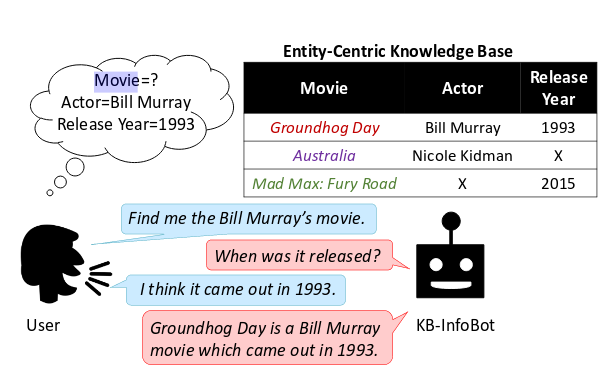
\includegraphics[width=0.5\linewidth]{pic/example.png}
  \caption{An example.}
  \label{fig:example}
\end{figure}
\paragraph{Methods}
Given conversation history and user utterance, KB-InfoBot uses Neural Belief Tracker to estimate the probability distribution $p^t_j$ and $q^t_j$ ($p^t_j$ is M multinomial distribution, $p^t_j(v), v\in V^j$ is the probability at turn t that the user constraint for slot $j$ is $v$. $q^t_j $ is a scalar probability of the user knowledge about the value of slot $j$, $q^t_j=Pr(\phi_j=1)$ indicates the probability that user knows the vaule of slot $j$). Then Soft-KB Lookup is used to estimate the probability $P^t_{\Gamma}(i)=Pr(G=i\vert U^t_1)$. $P^t_{\Gamma}(i)$ indicates the probability that user is interested in row $i$ of knowledge table, given utterance up to turn t. After that, the reuslt of Neural Belief Tracker and Soft-KB Lookup are summarized to internal state $s^t$. Finally, based on internal state $s^t$, we use Neural Policy Network to select an appropriate action $\pi$ from action set. The frame of this system is shown in figure \ref{fig:frame}.

\begin{figure}
   \centering
   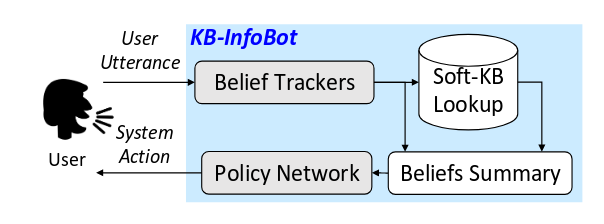
\includegraphics[width=0.5\linewidth]{pic/frame.png}
   \caption{system frame}
   \label{fig:frame}
\end{figure}
\paragraph{Techniques}
In this paper, author hopes to combine the result of Neural Belief Tracker (NBT) and the result of Soft-KB Lookup together by concatenating the results. However, the dimension is too large to combine the results together. Therefore, author decreases the dimension by extracting summary statistic, that is author uses entropy to represent a probability distribution. $s^t=[p^t_1,p^t_2,...,p^t_M,q^t_1,q^t_2,...,q^t_M,P^t_{\Gamma}]$ is internal state and element $p^t_j$ has $\vert V^j \vert$ dimensions. Therefore $s^t$ has $\sum_j \vert V^j \vert + 2M+N$ dimensions. For each slot $j$, we compute $\hat{p}^t_j(v)=w^t_j(v)\propto \sum_{i:T_{i,j}=v}P^t_{\Gamma}(i)+p^0_j\sum_{i:T_{i,j}=\phi}P^t_{\Gamma}(i)$ and then use the entropy of this new distribution $H(\hat{p}^t_j)$to represent the original distribution $p^t_j$. Finally the total dimension is decreased to $2M+1$.
\section{Details}
\subsection{Neural Belief Tracker(NBT)}
The NBT is implemented by a GRU neural network. The input to this network is the utterance from beginning to turn $t$. The internal state $h^t_j \in R^d=GRU(x_1,...,x_t)$ represents a summary of what the user has said about slot $j$ till turn $t$, note $h^0_j=0$. The belief state can be expressed as following:
\begin{equation}
p^t_j=softmax(W^p_j h^t_j +b^p_j) \mbox{, where  $W^p_j \in R^{V^j\times d}$, $b^p_j\in R^{V^j}$}
\end{equation}
\begin{equation}
q^t_j=\delta(W^q_j h^t_j +b^q_j) \mbox{, where  $W^q_j \in R^{1\times d}$, $b^p_j\in R$}
\end{equation}
\subsection{Soft-KB Lookup}
Soft-KB Lookup is used to determine the probability that the entity in which user is interested is row $i$ of KB tabele, entity $i$. 
\begin{equation}
P^t_{\Gamma}(i)=Pr(G=i\vert U^t_1) \propto \prod^M_j Pr(G_j=i\vert U^t_1)
\end{equation}
where $G$ means that the user's goal or intention, $G_j=i$ menans that with respect to the slot $j$, user is interested in row $i$. The prior distribution of $G$ is uniform distribution $G\sim U[\{1,2,...,N\}]$.
\begin{equation}
\begin{split}
&  P(G_j=i\vert U^t_1)\\
& =\sum^1_0 Pr(G_j=i,\phi_j=\phi\vert U^t_1)\\
& =\sum^1_0 Pr(G_j=i\vert \phi_j=\phi, U^t_1)Pr(\phi_j=\phi\vert U^t_1)\\
& =q^t_j Pr(G_j=i\vert \phi_j=1)+(1-q^t_j)Pr(G_j=i\vert \phi_j=0)
\end{split}
\end{equation}
\begin{equation}
Pr(G_j=i\vert \phi_j=0)=\frac{1}{N}
\end{equation}
where $\phi_j=0$ means that user doesn't know the value of slot $j$
\begin{equation}
Pr(G_j=i\vert \phi_j=1)=\left \{\begin{array}{ll}
\frac{1}{N} & \mbox{ $i\in M_j$}\\
\frac{p^t_j(v)}{N^v_j}(1-\frac{\vert M_j \vert}{N}) & \mbox{ $i\in M_j$} 
\end{array} \right.
\end{equation}
where $M_j$ is a set which includes all rows $i$ whose value of slot $j$ is missing.
\subsection{Neural Policy Network}
Here author uses GRU neural network to construct a Neural Policy Network which converts internal state $s^t$ to a probability distribution over the action set $\pi$.
\begin{equation}
\begin{split}
& h^t_{\pi}=GRU(s^1,...,s^t)\\
& \pi=softmax(W^{\pi}h^t_{\pi}+b^{\pi})
\end{split}
\end{equation}
Refer the paper \cite{DBLP:journals/corr/DhingraLLGCAD16}
\bibliography{test}
\end{document}
